\section{DONUT: \underline{D}ataset \underline{O}f ma\underline{N}ifold str\underline{U}c\underline{T}ures}
\label{sec:topogen}

\begin{figure}[t]
  \centering
  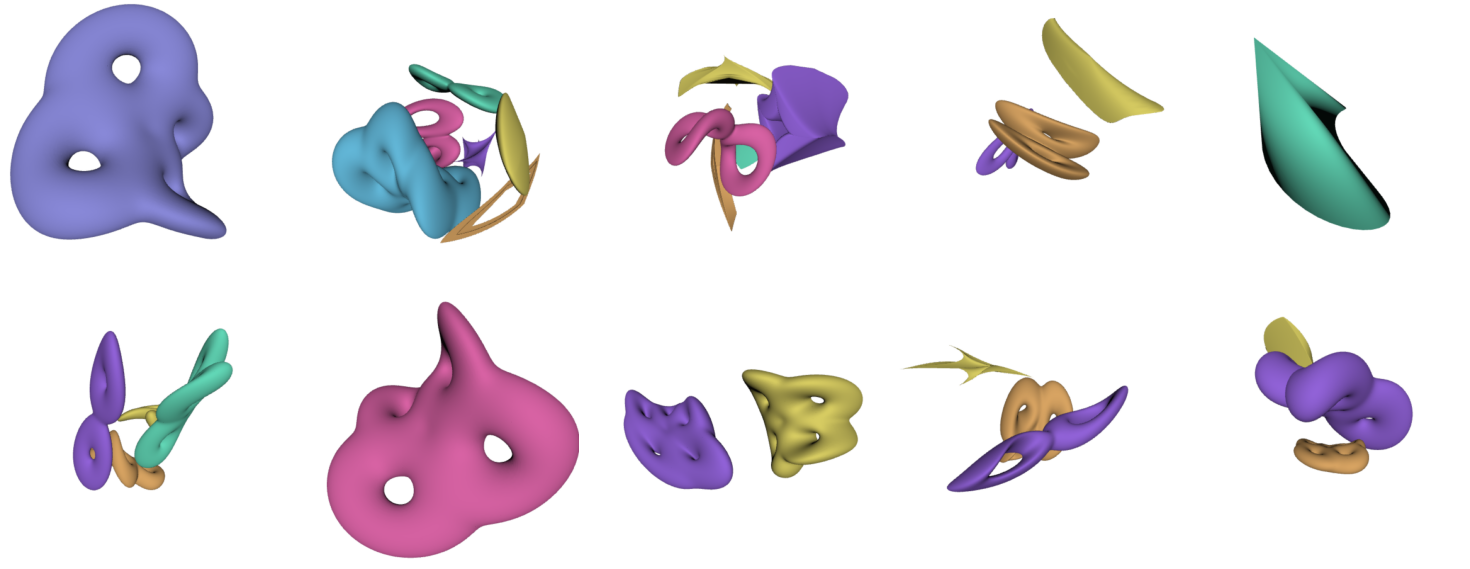
\includegraphics[width=1.0\linewidth]{figs/topogen/samples_overview.png}

  \label{fig:topogen-samples}
  \caption{\textbf{Random samples from the dataset.} Despite the fact that each sample is generated from a rather small family of shapes, both the topology preserving placement and augmentations allow for a rich variety of shapes, while ensuring topological consistency.}
  \label{fig:short}
\end{figure}


Understanding how models capture topological properties of 3D shapes is a key step toward disentangling geometric representation learning from semantic categorization. Existing 3D datasets, such as Objaverse~\cite{objaverse,objaverse_xl} or ShapeNet~\cite{shapenet}, primarily organize data by semantic class or surface geometry, without systematic control of topology. Probing topology-aware representations therefore requires datasets that expose explicit topological labels under controlled geometric variability.

To address this, we introduce DONUT, a scalable dataset of synthetic 3D shapes annotated with precise and balanced topological labels. Unlike prior datasets, DONUT is built from parametric families that guarantee topological correctness while enabling high geometric diversity. This design allows principled evaluation of how models represent intrinsic topological invariants such as connected components and genus.

\subsection{Existing datasets}
\label{ssec:existing_datasets}

Existing 3D datasets provide only limited support for probing whether models capture topological structure. Broadly, they fall into three categories: combinatorial-only benchmarks, geometric datasets with noisy topology, and synthetic datasets with limited diversity.

\paragraph{Combinatorial benchmarks.}
The MANTRA dataset (Manifold Triangulation Assemblage) \cite{mantra} provides combinatorial triangulations of 2D and 3D manifolds, represented as abstract simplicial complexes without embedding in $\mathbb{R}^3$. MANTRA is a valuable testbed for assessing whether graph- or simplicial complex models capture higher-order structures such as Betti numbers $(\beta_0, \beta_1, \beta_2)$. However, since it lacks any geometric realization, MANTRA is not suitable for evaluating models built on geometric 3D representations such as meshes, point clouds, or implicit fields.

\begin{table}[h]
  \begin{center}
  \begin{tabular}{l l l l r}
  Dataset & \#Samples & \rotatebox[origin=lB]{90}{Meshes} & \rotatebox[origin=lB]{90}{Manifold} & \rotatebox[origin=lB]{90}{Balanced annot.}\\
  \midrule
  \rowcolor{green!20}
  \multicolumn{1}{l|}{DONUT}  & 30,000   & \cm & \cm & \cm \\
  \multicolumn{1}{l|}{MANTRA \cite{mantra}} & 43,100 & -- & \cm & -- \\
  \multicolumn{1}{l|}{ABC \cite{abc}} & 1,000,000+ & \cm & --   & -- \\
  \multicolumn{1}{l|}{Thingi10K \cite{thingi}} & 10,000 & \cm & -- & -- \\
  \rowcolor{green!20}
  \multicolumn{1}{l|}{EuLearn  \cite{eulearn}} & 3,300 & \cm & \cm & \cm \\
  \midrule
  \end{tabular}
  \end{center}
  \vspace{-2mm}
  \caption{\textbf{Overview of existing datasets and their capabilities.} We summarize here the main characteristics of existing datasets with topological annotations. Besides EuLearn, all existing datasets with topological annotations come with downsides, discussed in Section~\ref{ssec:existing_datasets}. However, since EuLearn seems to be the most promising dataset, we carried out an extensive analysis to (1) highlight limitations that make it unreliable for further experiments and (2) motivate the use of DONUT (see Appendix~\ref{ssec:suppl_eulearn_analysis}). \textit{Note:} The number of samples for MANTRA only takes into account 2-manifolds.}
  \label{tab:datasets}
\end{table}

\paragraph{Geometric datasets with noisy topology.}
Large mesh datasets such as Thingi10K~\cite{thingi}, Objaverse~\cite{objaverse} and ABC~\cite{abc} contain CAD models and artistic objects, and include coarse topological annotations (number of components, genus). However, these annotations are unreliable for several reasons:

\begin{enumerate}
  \item \textit{Discrepancy between raw and perceptual components.} Artistic and CAD models are typically constructed from many sub-meshes, so the annotated component count often diverges from the semantically meaningful object count.
  \item \textit{Severe class imbalance.} While a wide range of genus values is theoretically possible, the overwhelming majority of meshes in both datasets have genus 0–2, making them unsuitable for balanced probing tasks.
  \item \textit{Structural artifacts.} Many meshes are non-manifold or self-intersecting, rendering quantities such as the Euler characteristic ill-defined:
\begin{equation}
  \chi = V - E + F = 2 - 2g - b + c
  \label{eq:euler}
\end{equation}

where $V,E,F$ are the number of vertices, edges, and faces, $g$ is genus, $b$ the number of boundary components, and $c$ the number of connected components.
Attempts to repair such meshes (e.g., Manifold~\cite{manifold}, ManifoldPlus~\cite{manifoldplus}, DOGN~\cite{dogn}, CLAY~\cite{clay}) face tradeoffs between oversmoothing geometry, introducing artifacts, or incurring prohibitive computational cost. As a result, these datasets cannot provide reliable large-scale topological ground truth.
\end{enumerate}

\paragraph{Synthetic datasets with limited diversity.} 
The EuLearn dataset~\cite{eulearn} addresses class imbalance by generating surfaces of varying genus from Fourier curves. While balanced across genera, EuLearn suffers from two critical issues: (i) samples within each genus class lack diversity, making them nearly indistinguishable, and (ii) strong correlations emerge between genus and canonical orientation, enabling trivial classification via nearest-neighbor with Chamfer distance. Consequently, EuLearn fails to disentangle topological structure from geometric shortcuts, limiting its usefulness for robust probing.

\begin{figure}[h]
  \centering
  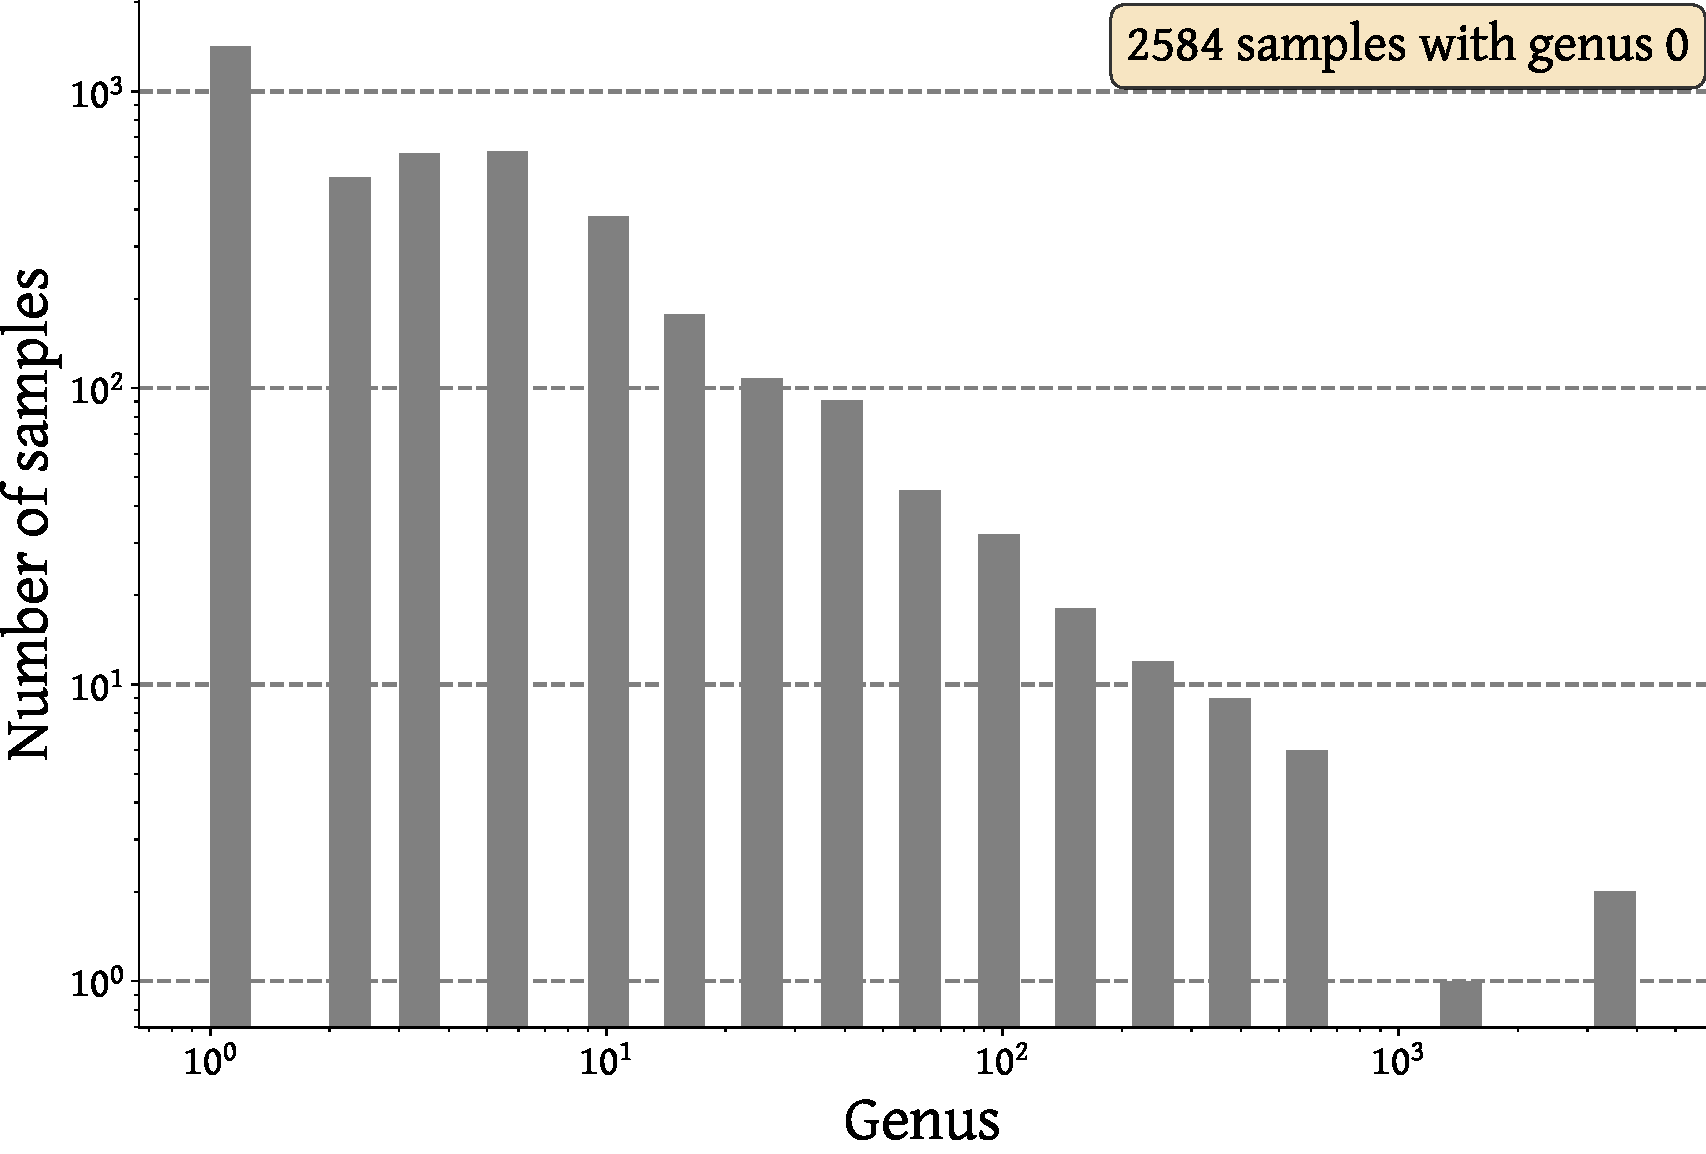
\includegraphics[width=0.5\linewidth]{figs/topogen/thingi_genus_hist.pdf}
   \caption{\textbf{Genus distribution of Thingi10K.} Both axes are plotted in log scale. The genus was estimated from the Euler characteristic, provided as metadata with the dataset; however, 2,651 samples do not fulfill the requirements to directly compute the genus from the Euler characteristic (see \ref{eq:euler}). They are therefore not taken into account here. The histogram shows that a large fraction of the dataset (over 3,000 samples out of 7,344) has genera of 0 or 1, indicating that higher-genus components are significantly underrepresented, which may limit accurate classification and probing analyses for those cases.}
   \label{fig:thingi-genus}
\end{figure}

\begin{figure}[h]
  \centering
  \includegraphics[width=0.5\linewidth]{figs/eulearn/dataset_samples.pdf}
   \caption{\textbf{Samples from the EuLearn dataset across different genera.} As the genus increases, shapes become geometrically more complex. This trend highlights a confounding factor in the dataset: geometric complexity grows together with genus. As a result, classification performance may be driven not only by topological information but also by correlated geometric cues.}
   \label{fig:eulearn-samples}
\end{figure}


\subsection{Method}
\label{ssec:topogen-method}

\begin{figure}[t]
  \centering
  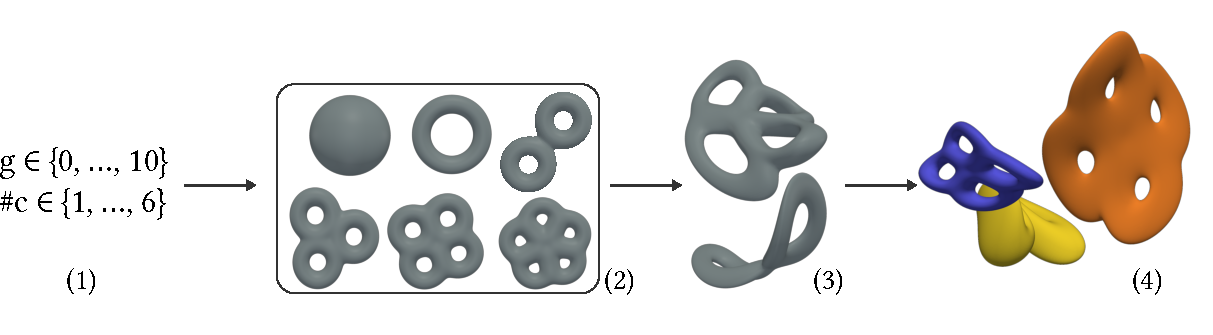
\includegraphics[width=1.0\linewidth]{figs/topogen/topogen_gen.pdf}
   \caption{\textbf{Generation Process Overview.} (1) For each sample, we pick a target genus and number of connected components. (Section~\ref{sssec:labels-distribution}) (2) We then distribute these values across a set of template shapes (Section~\ref{sssec:sample-level-properties}). (3) Each mesh is instantiated by sampling parameters from its parametric expression, and individually warped to bring more geometric diversity. (4) Finally, we apply a series of topology-preserving augmentations to increase geometric diversity while maintaining the original topological labels, and compose the final sample by merging all meshes. (Section~\ref{sssec:mesh-generation})}
   \label{fig:topogen-overview}
\end{figure}

Since DONUT is made of synthetic shapes, two critical challenges must be addressed to ensure that the results obtained from this dataset are relevant. 1) Foundation models are pretrained on real shapes. Therefore, learned features reflect the distribution of real world geometry and semantics. Synthetic data, however, introduce patterns and biases that don't exist in real data, making them fall out-of-distribution. 2) Another common pitfall of synthetic datasets (cf. EuLearn) is the lack of variability, making evluation tasks such as probing, trivial. The first challenge is mitigated because pretrained foundation models (e.g., on ShapeNet or Objaverse) already encompass a wide range of synthetic geometries, keeping DONUT samples within their learned data distribution. This is experimentally validated in Figure (+ figure with umaps). To address the second challenge, we developed a set of rules and augmentation techniques to ensure that the generated shapes are both diverse and topologically accurate.

The generation process was designed to jointly satisfy three criteria: (i) exact control of topology, (ii) high geometric diversity, and (iii) scalability to tens of thousands of shapes. Figure \ref{fig:topogen-overview} provides an overview of the generation pipeline, which we now describe in detail.

\subsubsection{Topological Control}
\label{sssec:labels-distribution}

A central design choice in DONUT is to ensure balanced topological supervision across the dataset. To this end, both the genus and the number of connected components are sampled such that their marginal distributions are approximately uniform. This prevents any single topological class from dominating and guarantees that models trained on the dataset are exposed to the full spectrum of topological structures. We bring this guarantee over marginal distributions by first sampling the labels before actually generating any mesh. \ref{sec:topogen-complements} formally describes how the labels are sampled and further details the properties of the dataset we used for all our experiments

Each sample is further composed of multiple meshes selected from a predefined family of template shapes. This choice introduces large geometric variability while maintaining strict control over label balance. As a result, the dataset couples statistical uniformity in labels with broad diversity in shape realizations. Nevertheless, by limiting ourselves to certain families of geometric shapes, we avoided falling into the pitfall of geometric complexity mentioned earlier. 

\subsubsection{Geometric Diversity}
\label{sssec:sample-level-properties}

At the level of individual samples, the generation process begins by selecting the global genus and number of connected components. These values are then distributed across the meshes composing the sample. For example, a sample may include one mesh of genus one, several genus-zero meshes, or even higher-genus meshes, depending on the chosen configuration.

Each mesh is then instantiated from a specific parametric family of shapes:
\begin{itemize}
  \item \textit{Genus 0:} Superellipsoids and cones
  \item \textit{Genus 1:} Supertoroids and cones
  \item \textit{Genus $\geq 2$:} K-tori
\end{itemize}

\textbf{Superquadrics.} Superellipsoids  (resp. toroids) are part of a wider family of parametric shapes called superquadrics. They were introduced by Barr et al. \cite{superquadrics} in 1981 and are widely used in computer graphics for their ability to represent a large range of shapes with a small number of compact parameters. Superquadrics have recently regained attention in 3D scene understanding, notably in SuperDec \cite{superdec}, because of their expressiveness and their ability to approximate complex structures by composition. Their implicit equation is given by:

\begin{equation}
\left( \left| \frac{x}{s_x} \right|^{\tfrac{2}{\epsilon_2}}
     + \left| \frac{y}{s_y} \right|^{\tfrac{2}{\epsilon_2}} \right)^{\tfrac{\epsilon_2}{\epsilon_1}}
+ \left| \frac{z}{s_z} \right|^{\tfrac{2}{\epsilon_1}}
= 1
\end{equation}

where $(s_x, s_y, s_z) > 0$ are scale factors along the $x, y, z$ axes respectively, and $(\epsilon_1, \epsilon_2) > 0$ are shape exponents that modulate the surface's roundness (resp. sharpness). Sampling these parameters within predefined ranges allows to efficiently sample a variety of shapes while maintaining control over their topological properties.

\subsubsection{Scalability}
\label{sssec:mesh-generation}

One key challenge is to be able to generate a large amount of samples (up to $10^5$) in a reasonable amount of time. This order of magnitude is motivated the results of Point-MAE-Zero \cite{pmaezero}. Accurate representations were obtained with a pretraining set containing around 150K samples. While we further use DONUT essentially for evaluation/probing tasks, we want to preserve the possibility of scaling to pretraining regimes where data requirements are significantly higher. We therefore minimize computationally intensive operations. k-tori aside, every mesh is generated either with its parametric expression when available, or with simple rules.

\paragraph{Cones.} \dots

\paragraph{Superquadrics.} Meshes corresponding to super ellipsoids and super toroids are generated directly from their parametric forms. The procedure consists of two steps: 1) generate a base template mesh (a sphere for ellipsoids, a torus for toroids) where vertices are expressed in spherical (resp. toroidal) coordinates, and 2) deform it according to the superquadric equations. This construction is lightweight, parallelizable, and supports fast large-scale dataset generation. The parametric equations we use in practice are as follows:
\begin{equation}
\begin{aligned}
\text{Ellipsoid} \quad
\begin{cases}
x(u,v) &= s_x \, C_{\epsilon_1}(v) \, C_{\epsilon_2}(u) \\
y(u,v) &= s_y \, S_{\epsilon_1}(v) \, S_{\epsilon_2}(u) \\
z(u,v) &= s_z \, S_{\epsilon_1}(v)
\end{cases}
\end{aligned}
\qquad
\begin{aligned}
\text{Toroid} \quad
\begin{cases}
x(u,v) &= s_x \, \bigl(R + C_{\epsilon_1}(v)\bigr) \, C_{\epsilon_2}(u) \\
y(u,v) &= s_y \, \bigl(R + S_{\epsilon_1}(v)\bigr) \, S_{\epsilon_2}(u) \\
z(u,v) &= s_z \, S_{\epsilon_1}(v)
\end{cases}
\end{aligned}
\end{equation}


where $u,v \in [-\pi, \pi]$ are the vertex coordinates of the template mesh is spherical (resp. toroidal) coordinates and:

\begin{equation}
\begin{aligned}
C_\epsilon(u) &= \operatorname{sign}(\cos(u)) \, |\cos(u)|^\epsilon \\
S_\epsilon(u) &= \operatorname{sign}(\sin(u)) \, |\sin(u)|^\epsilon
\end{aligned}
\end{equation}


\begin{figure}[t]
  \centering
  \begin{subfigure}[t]{0.48\linewidth}
    \centering
    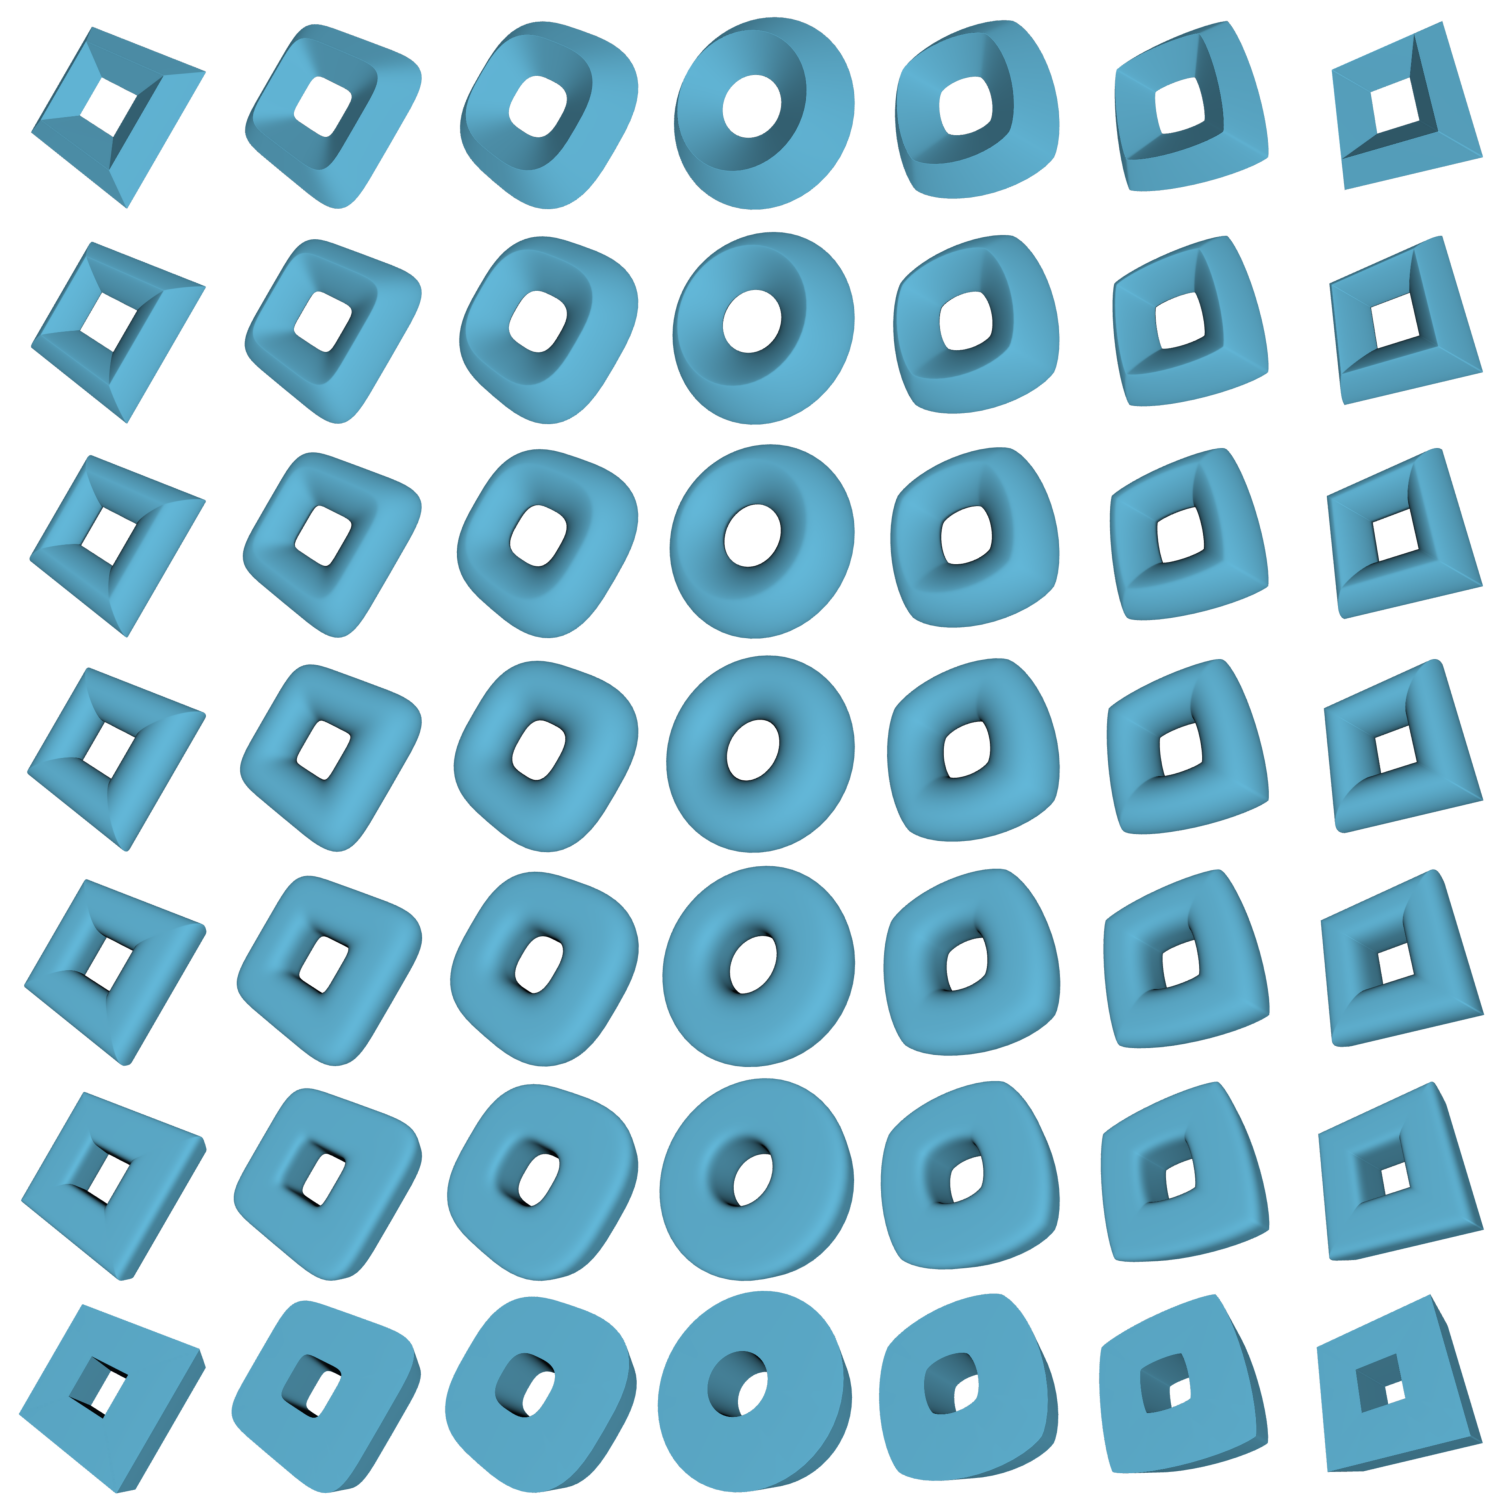
\includegraphics[width=\linewidth]{figs/topogen/toroids_overview.png}
    \caption{Supertoroids.}
    \label{fig:toroids-overview}
  \end{subfigure}
  \hfill
  \begin{subfigure}[t]{0.48\linewidth}
    \centering
    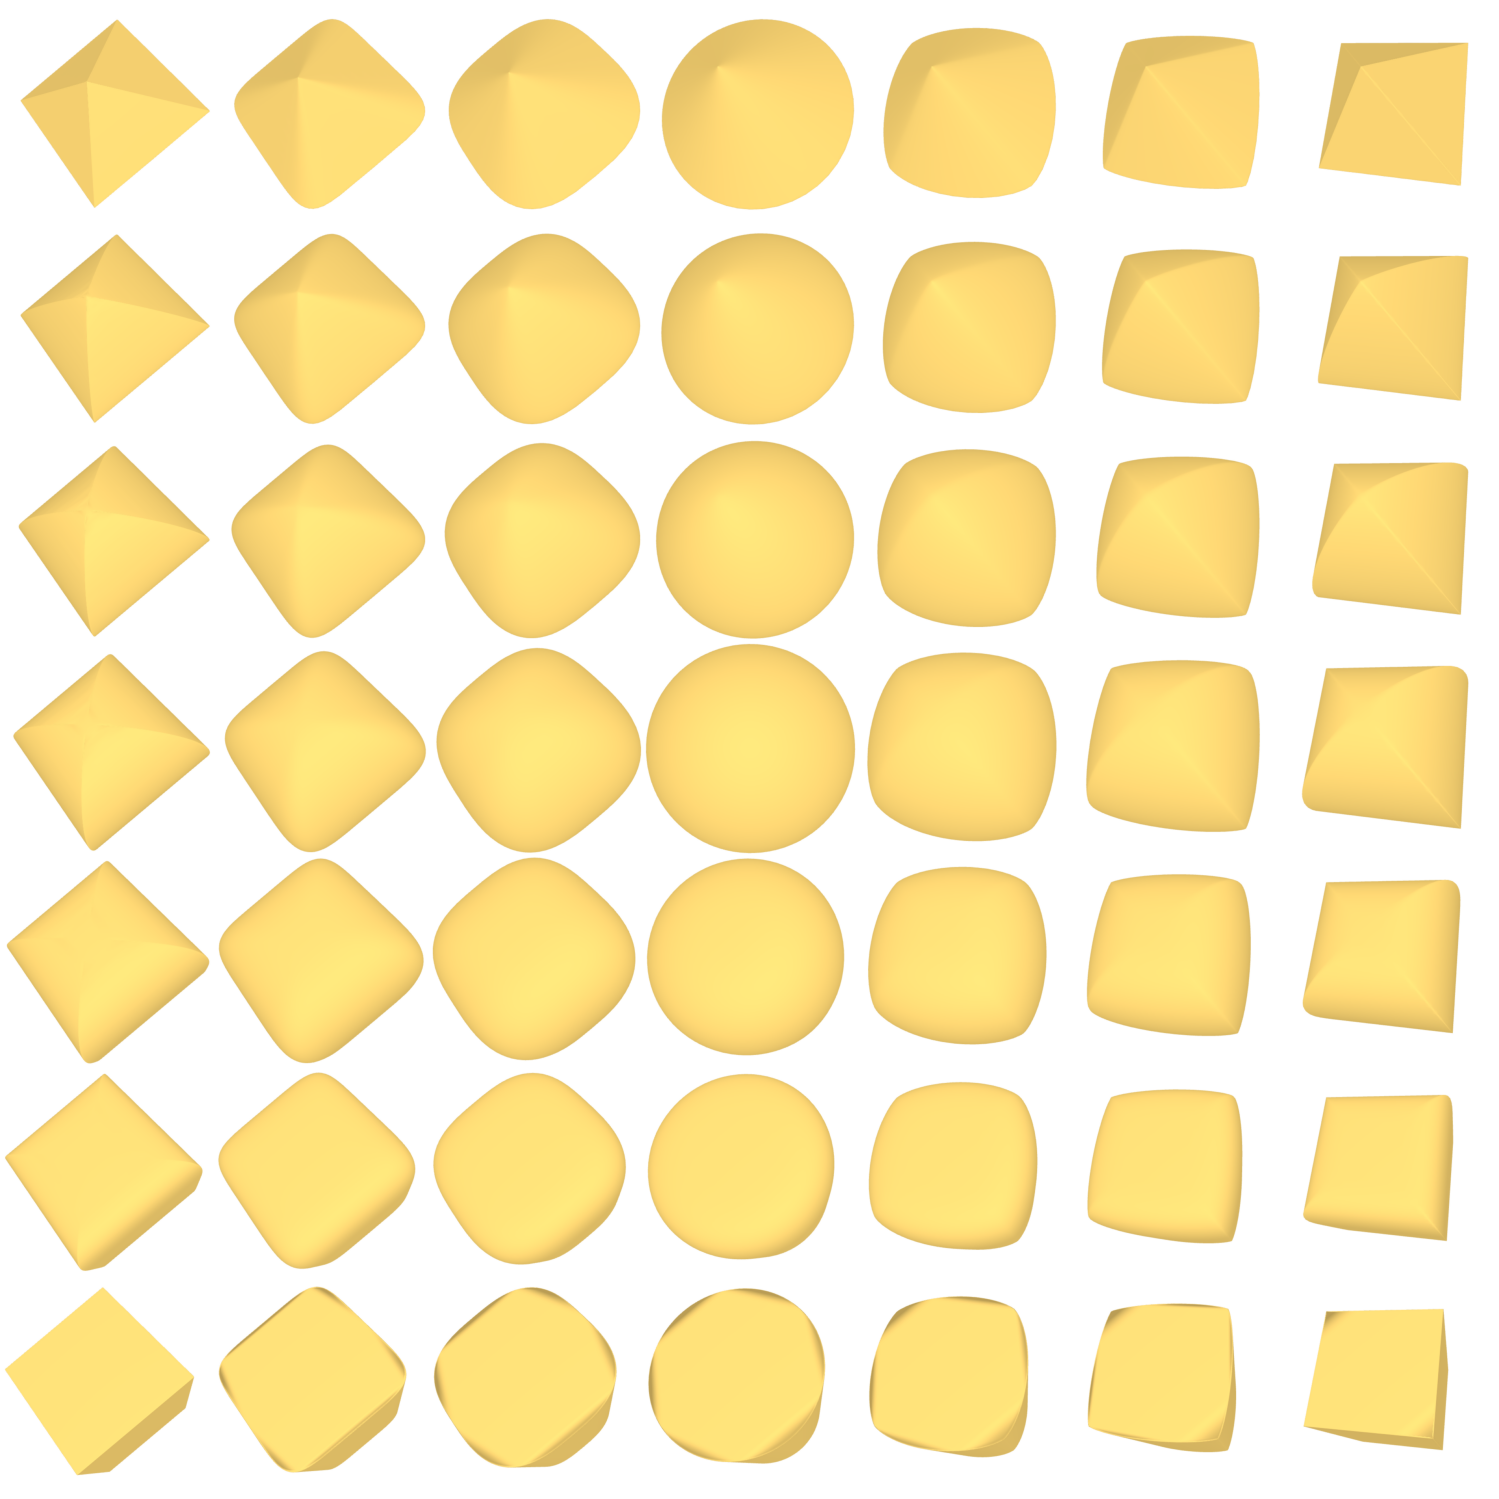
\includegraphics[width=\linewidth]{figs/topogen/ellipsoids_overview.png}
    \caption{Superellipsoids.}
    \label{fig:ellipsoids-overview}
  \end{subfigure}
  \caption{Overview of different shapes obtained for fixed values of $a_i, i \in \{1, 2, 3\}$ and increasing values of $\epsilon_1$ (left to right) and $\epsilon_2$ (bottom to top). 
  (a) Different supertoroids. As mentioned in TO ADD, using these shapes for $k$-tori ($k \geq 2$) is challenging because they may not preserve the genus, for instance if some parts are too thin or sharp. 
  (b) Different superellipsoids.}
  \label{fig:overview}
\end{figure}

\paragraph{$K$-tori.} In the case of higher-genus meshes, there are no closed-form parametric equations. Instead, we leverage the implicit formulation of tori. A $k$-torus is generated by (1) evenly distributing tori on a circle, (2) blending their signed distance functions (SDF) through a smooth union operator, and finally (3) extracting the mesh via marching cubes with a grid-size. However, this process is more computationally intensive as it requires applying marching cubes the discretized SDF, whose complexity scales in $O(N^3)$ where $N$ is the grid size. And since we seek to have high quality meshes to preserve fine-grained details (here holes), we use a higher grid resolution.

To smoothly blend the SDF of each torus generated independently, we use the \textit{smooth minimum} operator:

\begin{equation}
\operatorname{softmin}_k(s_1, s_2, \dots, s_n) 
= -\frac{1}{k} \log \left( \sum_{i=1}^n e^{-k s_i} \right)
\end{equation}

Where $(s_1, s_2, \dots, s_n) \in \mathbb{R}^{(N^3)}$ are the SDF of individual tori and $k$ is a hyperparameter controlling the smoothness of the blending. This operator is applied voxel wise. In other words, each voxel of the blended SDF is assigned with the smooth minimum value of the individual SDF.

\subsubsection{Topological Consistency and Diversity}
\label{sssec:top-consistency}

Two challenges remain to be addressed. First, when placing components within a sample, we must ensure they don't overlap. At the same time, they need to be close enough to make the samples both topologically consistent and challenging enough for models to correctly identify the number of connected components. In early experiments, we observed that if components are too far apart, the task can be trivially solved using a simple KNN classifier with Chamfer distance. Second, even with careful placement, models tend to overfit, sometimes even when using simple linear heads on top of learned features, showing that this alone is insufficient to evaluate their true topological understanding. To increase variability while preserving topological labels, we apply transformations both at the sample level and the individual component level.

\paragraph{Consistency.} 
To address the first challenge, we developed a two-stage placement procedure. Suppose there are already some components correctly placed within a sample. To add a new component, we first place it randomly in the sample and then check for intersections with the existing components. Experimentally, we observed that a randomly placed mesh overlaps with at most two other components. If the new component overlaps with only one existing component, we identify the point on the new mesh that is most deeply inside the other component and push the new component along the opposite direction of the surface normal at that point. For intricate shapes, a single adjustment may create new overlaps, so we repeat this step five times. If overlaps remain after five attempts, the component is discarded and a new one is generated and randomly placed. This iterative procedure improves efficiency: in practice, one or two adjustments are sufficient to resolve overlaps, making it faster than discarding and regenerating components immediately.

\paragraph{Variability.} 
To further increase the diversity of DONUT while preserving topological labels, we apply transformations both at the sample level and at the component level. Commonly used rigid transformations, such as rotations and scaling, are applied to both components and full samples. At the component level, we do not apply translations to avoid creating overlaps that would break the overall topology of the sample. To introduce additional geometric variability, we also apply twisting deformations (Figure \ref{fig:twisted-comparison}). Without loss of generality, we assume that a component (or a full sample) lies within the unit sphere, as global scaling can be applied afterward. First, we uniformly sample a direction on the unit sphere, which defines an axis for the twist. Next, we define a smooth scalar function along this axis that determines the rotation angle. Finally, each vertex is rotated around the axis by the angle given by the scalar function evaluated at the point where the vertex projects along the axis. This procedure introduces non-rigid variability while preserving the genus and connectivity of each component and of the overall sample.

\begin{figure}[t]
  \centering
  \begin{subfigure}[t]{0.48\linewidth}
    \centering
    \includegraphics[width=\linewidth]{figs/topogen/ktori_overview.png}
    \caption{\textbf{Degrees of freedom allowed on $k$-tori.} 
    Prior to the sequence of transformations applied to each individual component (e.g. rotation, twisting) we allow some variability during the generation. 
    The x-axis represents the ratio \textit{major radius / minor radius}. 
    The y-axis shows how the template shape is modified as we increase the value of $k$ (i.e. the genus). 
    \textit{Note:} In the actual dataset, $1$-tori are generated with the parametric representation of supertoroids, since a regular torus is a particular case of supertoroid. 
    However, for $k \geq 2$, using a composition of $1$-tori is more reliable. 
    Some parameter sets can lead to undesirable holes in the final shape.}
    \label{fig:ktori-overview}
  \end{subfigure}
  \hfill
  \begin{subfigure}[t]{0.48\linewidth}
    \centering
    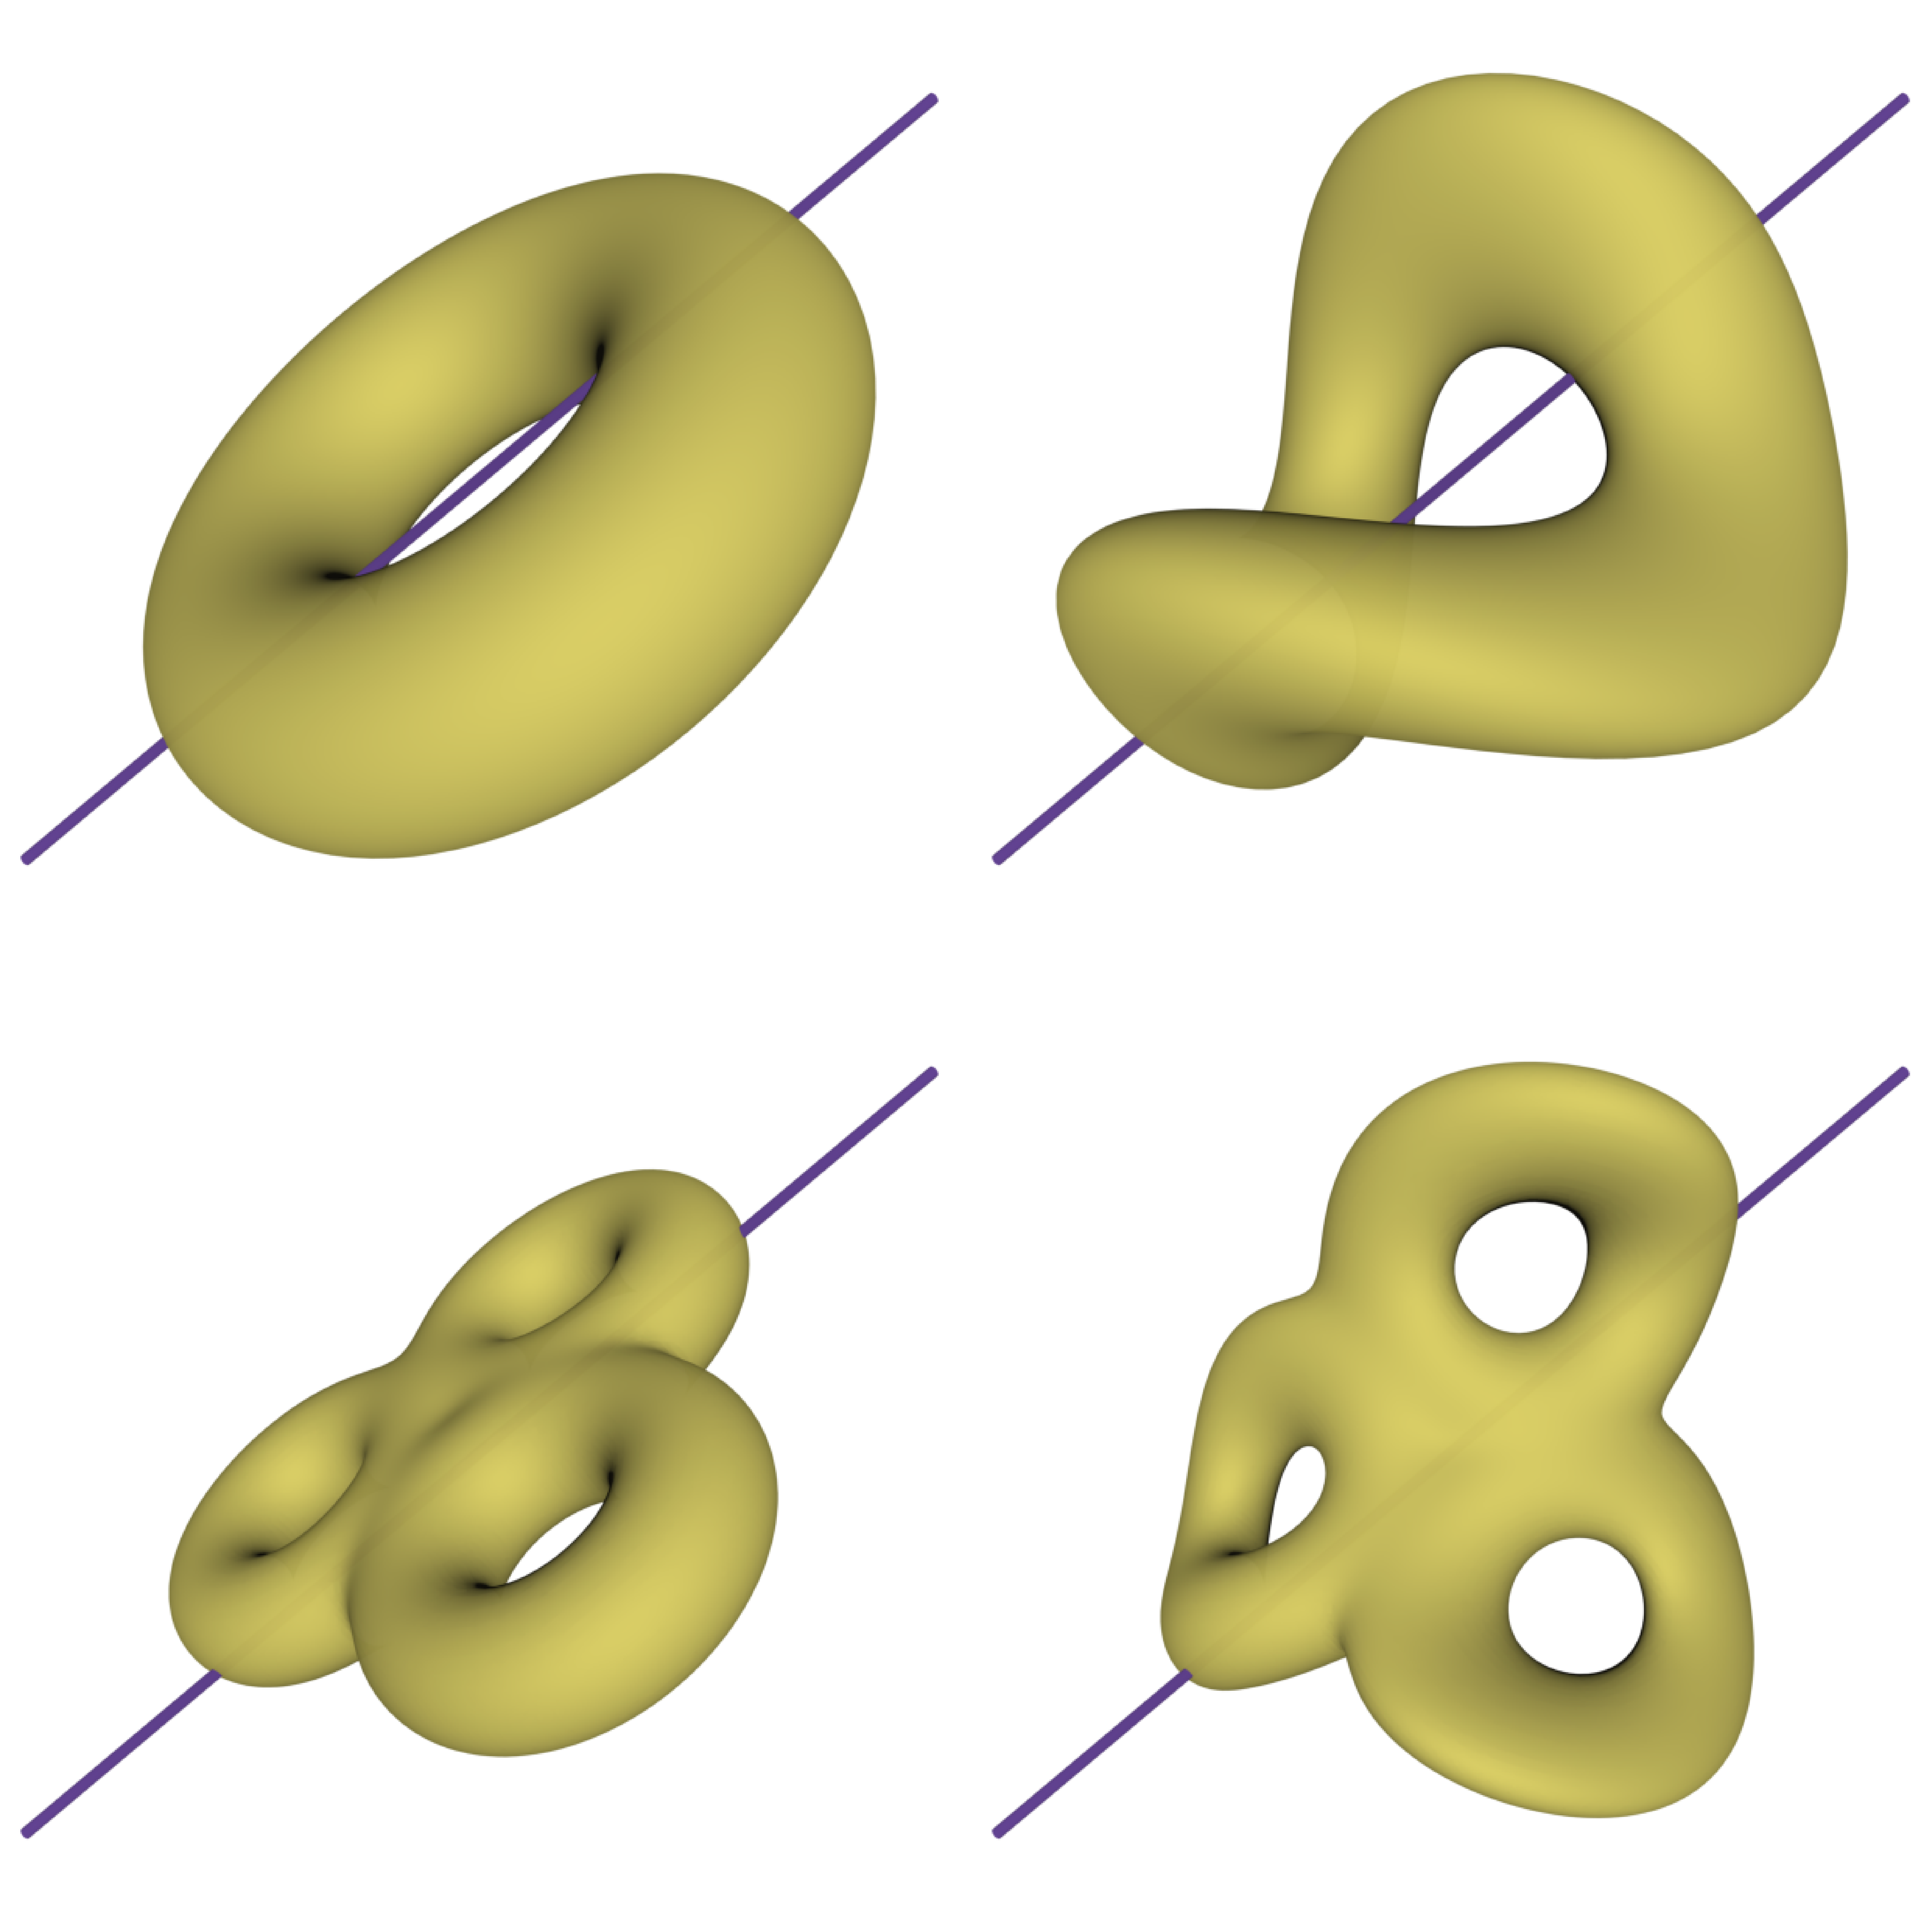
\includegraphics[width=\linewidth]{figs/topogen/twisted_comparison.png}
    \caption{\textbf{Effect of twisting.} 
    Original template shapes (left) are twisted along the purple axis (right). 
    Twisting deformations introduce non-rigid variability while preserving the genus and connectivity of each component. 
    Here the scalar function defined along the axis is affine between $-\pi/6$ and $\pi/3$. 
    We apply this augmentation at the component and sample level.}
    \label{fig:twisted-comparison}
  \end{subfigure}
\end{figure}

\subsection{Analysis}

This section provides a detailed characterization of DONUT. We first present dataset statistics, label distributions, and its relation to pretrained models. We then discuss baseline performance and introduce two complementary protocols designed to verify that models trained on DONUT actually capture topological features.

\subsubsection{General Properties}
\label{sssec:topogen-general-properties}

\paragraph{Dataset statistics.}
DONUT contains 29,517 samples divided into training, validation, and test splits of 80\%, 10\%, and 10\%. Each sample has between 1 and 6 connected components, with the total genus ranging from 0 to 10. A single component has genus at most 5 (corresponding to a 5-torus (Figure~\ref{fig:ktori-overview})). The dataset size was chosen to balance feasibility and reliability: smaller datasets led to overfitting while much larger datasets made experiments costly. Figure~\ref{fig:topogen-gen-comp-hist} reports the marginal distributions of genera and connected components.

\paragraph{Distributions and scalability.}
Figure~\ref{fig:topogen-umaps-overview} shows that synthetic samples from DONUT occupy the same representation space as training data used by common 3D encoders. This indicates that the dataset lies within the learned distribution of existing models rather than being out-of-distribution. In addition, Figure~\ref{fig:topogen-gen-time} reports the time required to generate different dataset sizes, showing that large-scale variants remain practical.

\subsubsection{Baselines and Transferability}
\label{sssec:topogen-transferability}

We trained several classical point-cloud models (PointNet, PointNet++, DGCNN) and recent persistence-based models (PersFormer, xPerT, PersLay) on DONUT. Results are reported in Table~\ref{tab:topogen-results}. Beyond in-distribution accuracy, a key question is whether these models actually capture topology or only rely on geometric characteristics.

Transferability provides a natural probe. To test this, we evaluated models on a curated subset of ABC. This set contains shapes whose geometry differs significantly from the training distribution, but whose topology is well characterized and within the label space. If models have learned topology, they should retain reasonable performance on ABC despite geometric differences. Table~\ref{tab:topogen-results} shows that DGCNN and specialized topological models maintain strong transfer, supporting the idea that DONUT encourages models to focus on topology. We note that weak transfer can also reflect limitations of current architectures rather than flaws in the dataset itself.

\begin{table}[h]
\centering
\begin{tabular}{l|ccc|ccc}
\toprule
 & \multicolumn{3}{c|}{\textbf{Genus}} & \multicolumn{3}{c}{\textbf{Connected Components}} \\
% \cmidrule{lr}{2-4} \cmidrule{lr}{5-7}
Model & MSE$\downarrow$ & Acc.$\uparrow$ & F1$\uparrow$ & MSE$\downarrow$ & Acc.$\uparrow$ & F1$\uparrow$ \\
\midrule
\multicolumn{1}{l}{} & \multicolumn{6}{c}{\textit{Point-based models}} \\
\midrule
PointNet~\cite{pointnet}   & 14.2/9.35 & 20.9/12.7 & 17.4/12.1 & 0.92/0.93 & 56.7/21.6 & 55.5/22.0 \\
PointNet++~\cite{pointnet++} &  -- & -- & -- & -- & -- & -- \\
Transformer (scratch) & -- & -- & -- & -- & -- & -- \\
Transformer (pretrained) & -- & -- & -- & -- & -- & -- \\
DGCNN~\cite{dgcnn}      & 1.05/11.7 & 51.5/18.1 & 51.3/15.2 & 0.11/1.04 & 89.1/27.7 & 89.1/25.4 \\
\midrule
\multicolumn{1}{l}{} & \multicolumn{6}{c}{\textit{Persistence-based models}} \\
\midrule
PersFormer~\cite{persformer} & -- & -- & -- & -- & -- & -- \\
xPerT~\cite{xpert}      & -- & -- & -- & -- & -- & -- \\
PersLay~\cite{perslay}    & -- & -- & -- & -- & -- & -- \\
\bottomrule
\end{tabular}
\caption{\textbf{Performance of baseline models trained on DONUT and evaluated both in-distribution and on ABC.} Values are reported as \textit{DONUT/ABC}. We report mean squared error (MSE), balanced accuracy (Acc.), and balanced F1-score (F1). MSE is reported to capture how far off predictions are from the ground-truth on average, which is particularly relevant given the natural hierarchy of the labels (genus and connected components): misclassifying by a larger margin is more severe than a closer miss. }
\label{tab:topogen-results}
\end{table}


\subsubsection{Saliency Analysis}
\label{sssec:topogen-saliency}

To further understand model behavior, we visualize saliency maps on toy shapes. These maps highlight which regions contribute most to predictions. When trained to predict genus, models tend to focus on cycles, while for connected components they concentrate around contact points between shapes (Figure~\ref{fig:dgcnn-saliency}). Such results suggest that models attend to meaningful topological structures rather than exploiting geometric shortcuts.

\begin{figure*}[t]
  \centering
  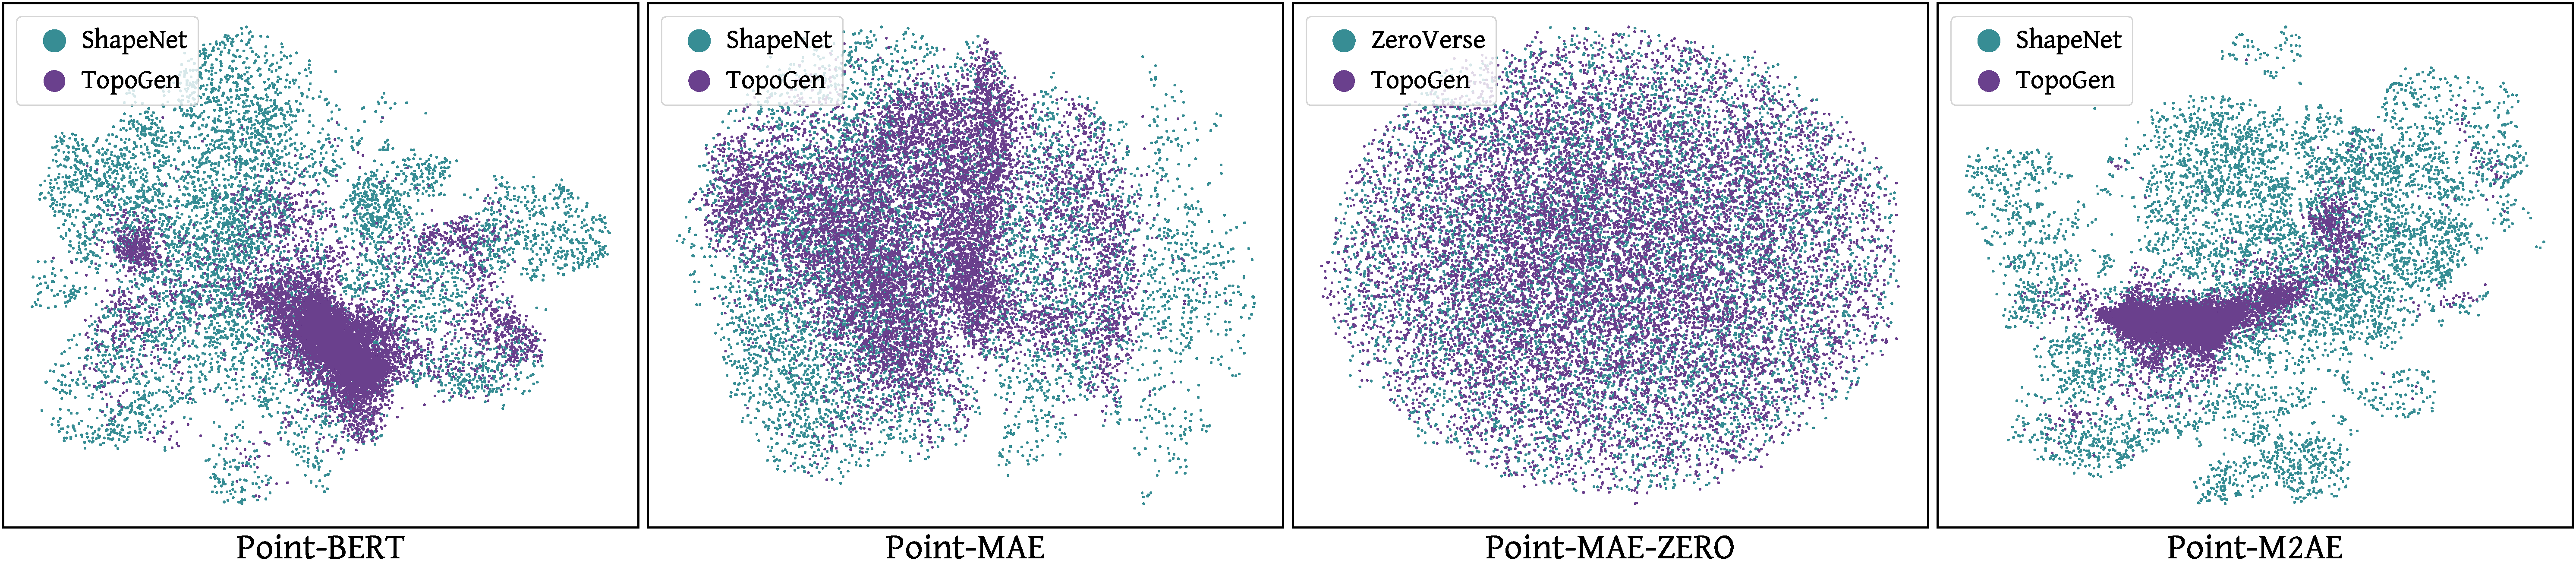
\includegraphics[width=\linewidth]{figs/topogen/umaps_overview.pdf}
  \caption{\textbf{UMAP embeddings of features learned by 3D encoders.} DONUT samples project into the same space as the original training data, indicating that they are not out-of-distribution.}
  \label{fig:topogen-umaps-overview}
\end{figure*}


\begin{figure}[t!]
  \centering
  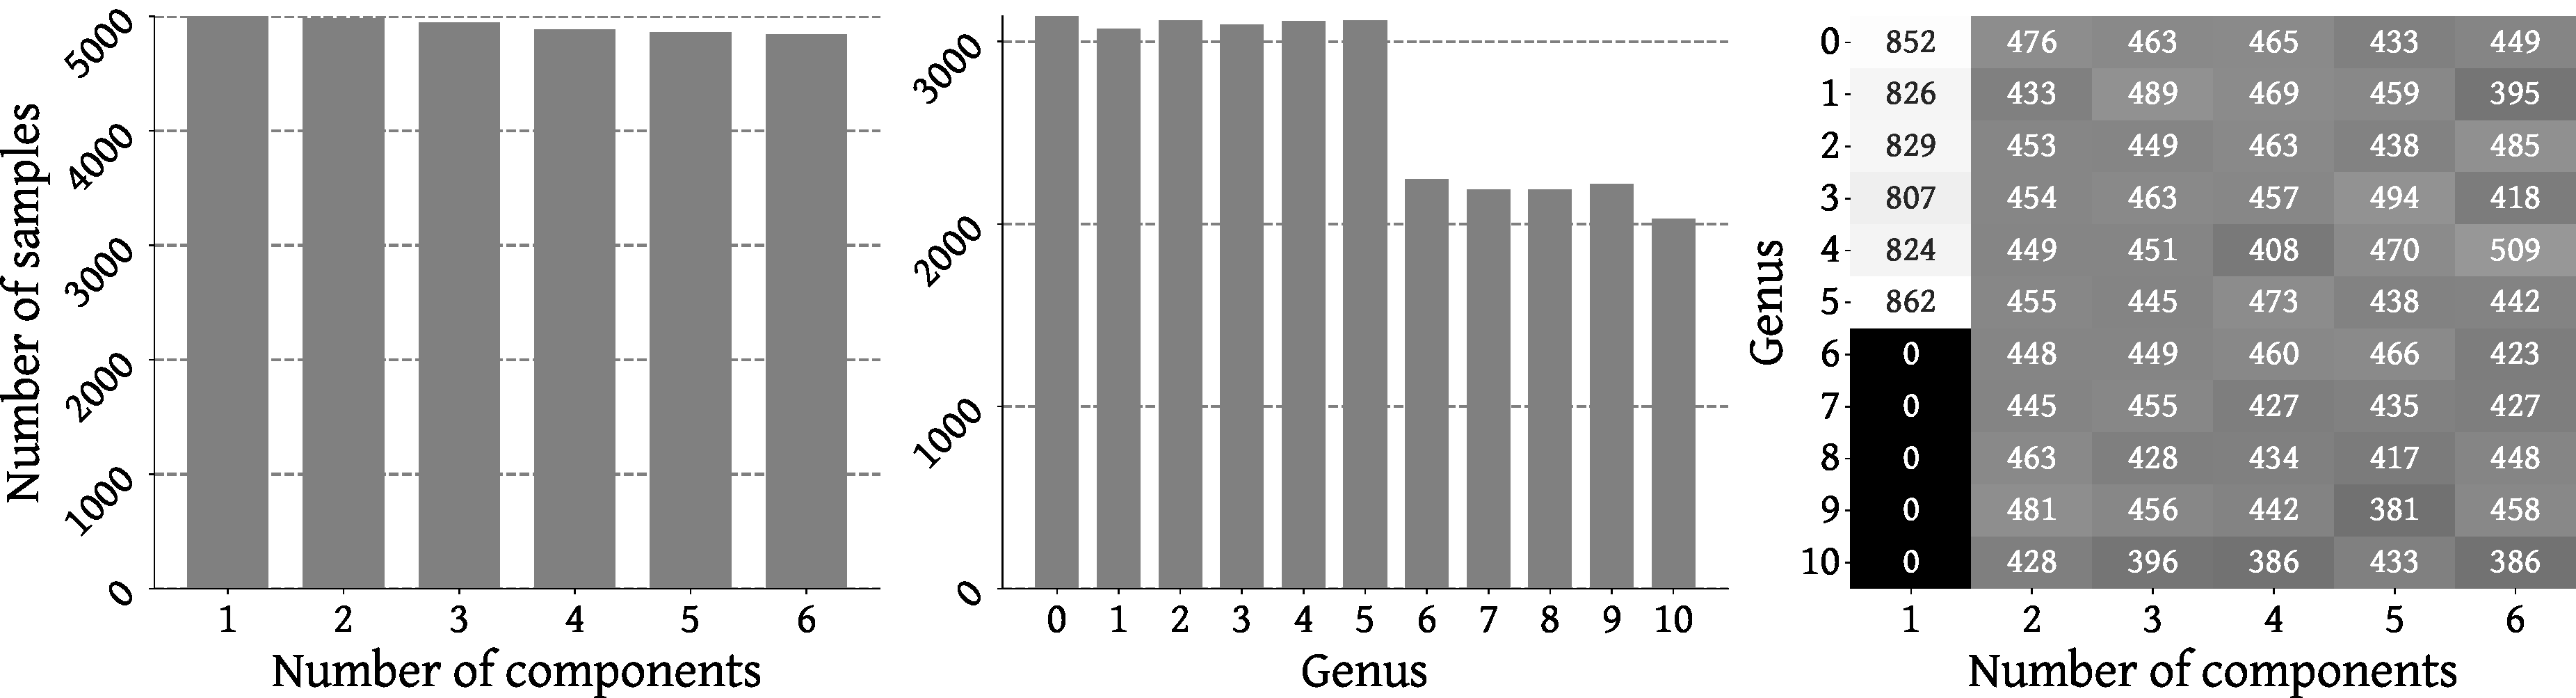
\includegraphics[width=\linewidth]{figs/topogen/label_distribution.pdf}
  \caption{\textbf{Label distributions for genus and connected components.} The marginal distributions of genus and connected components (left and middle histograms) are approximately uniform, ensuring balanced supervision across topological classes. The right plot shows the joint distribution. The absence of samples with one connected component and genus greater than 5 stems from the constraints of our generation process, which limits individual components to a maximum genus of 5. The only way to achieve a genus greater than 5 is by combining multiple components.}
  \label{fig:topogen-properties}
\end{figure}

% \begin{figure}[t]
%   \centering
%   \begin{subfigure}[t]{0.66\linewidth}
%     \centering
%     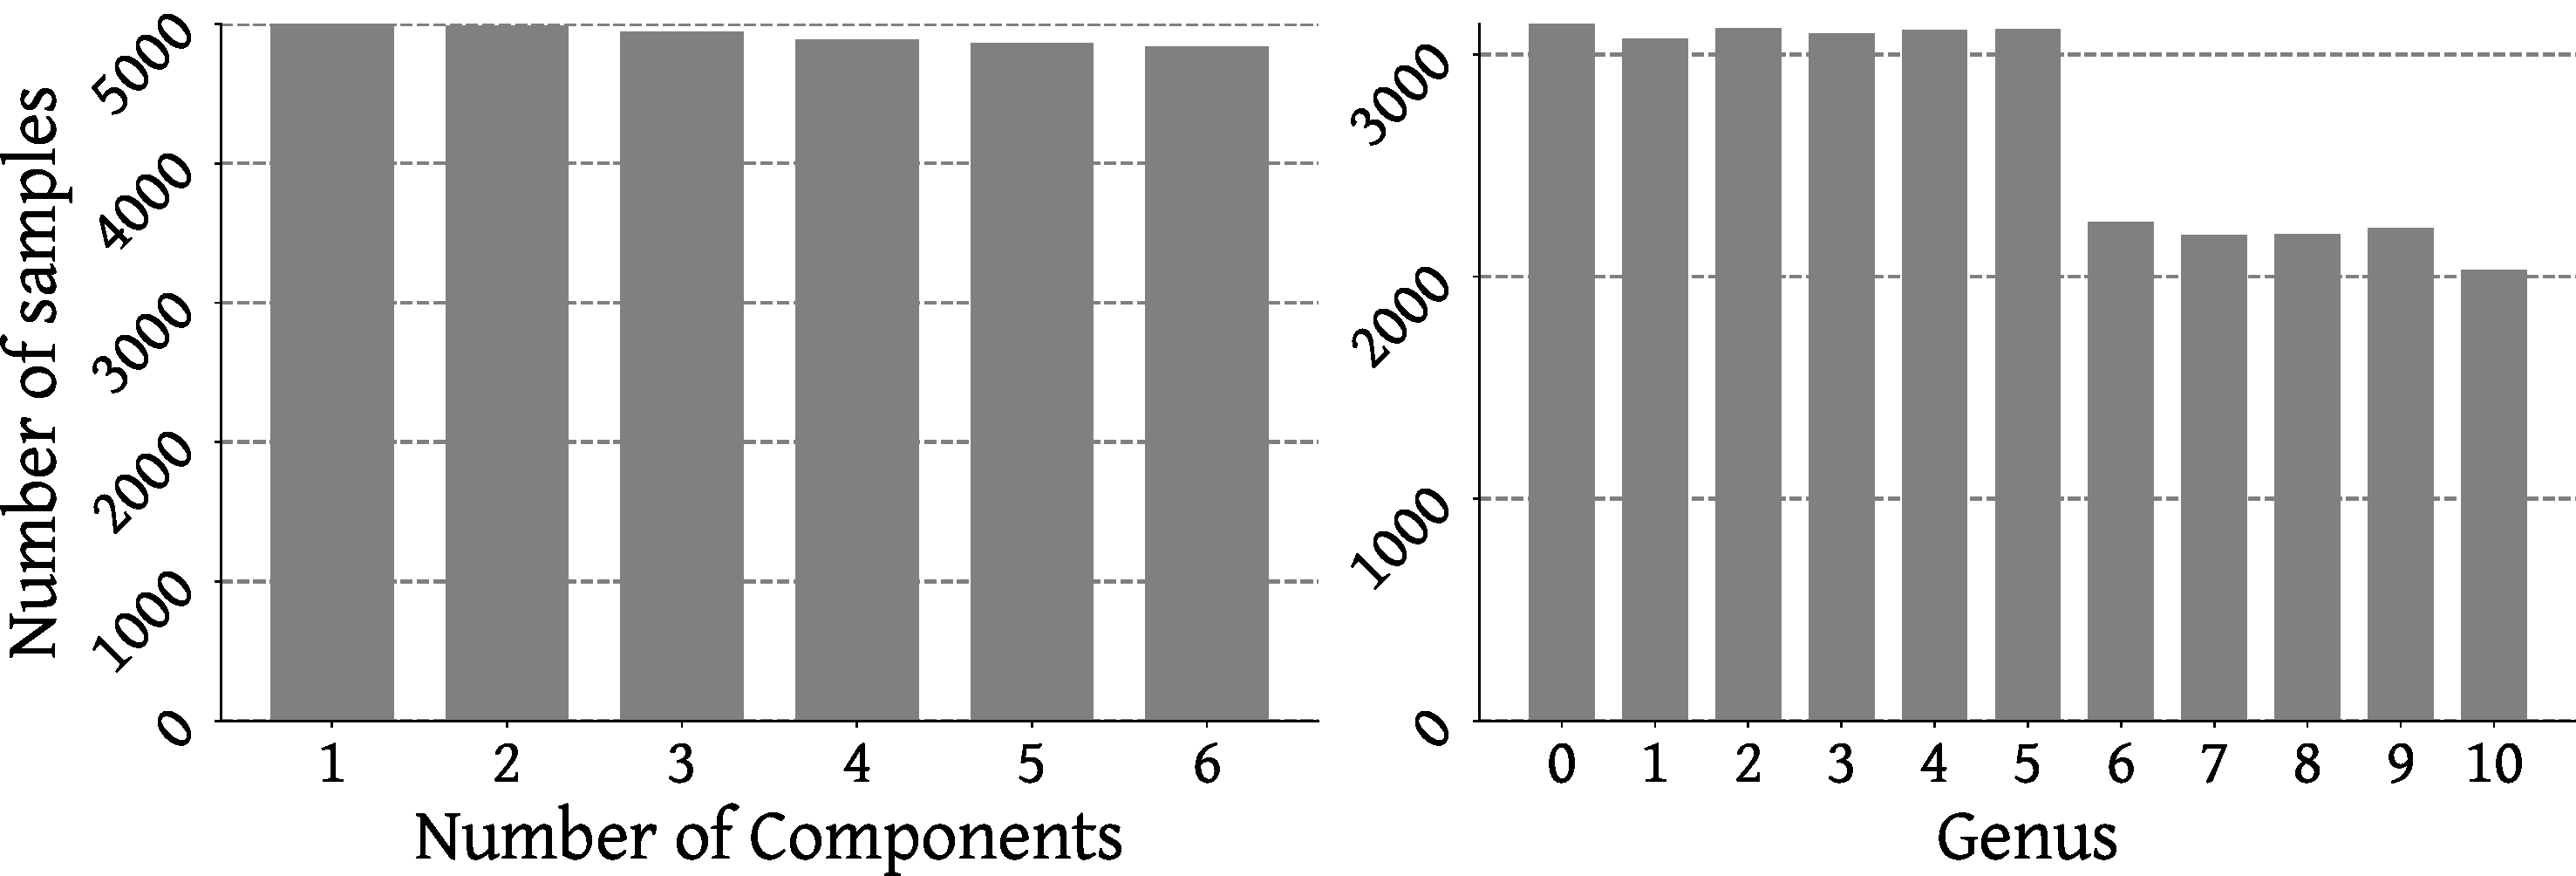
\includegraphics[width=\linewidth]{figs/topogen/components_genus_hist.pdf}
%     \caption{Label distributions for genus and connected components.}
%     \label{fig:topogen-gen-comp-hist}
%   \end{subfigure}%
%   \hfill
%   \begin{subfigure}[t]{0.33\linewidth}
%     \centering
%     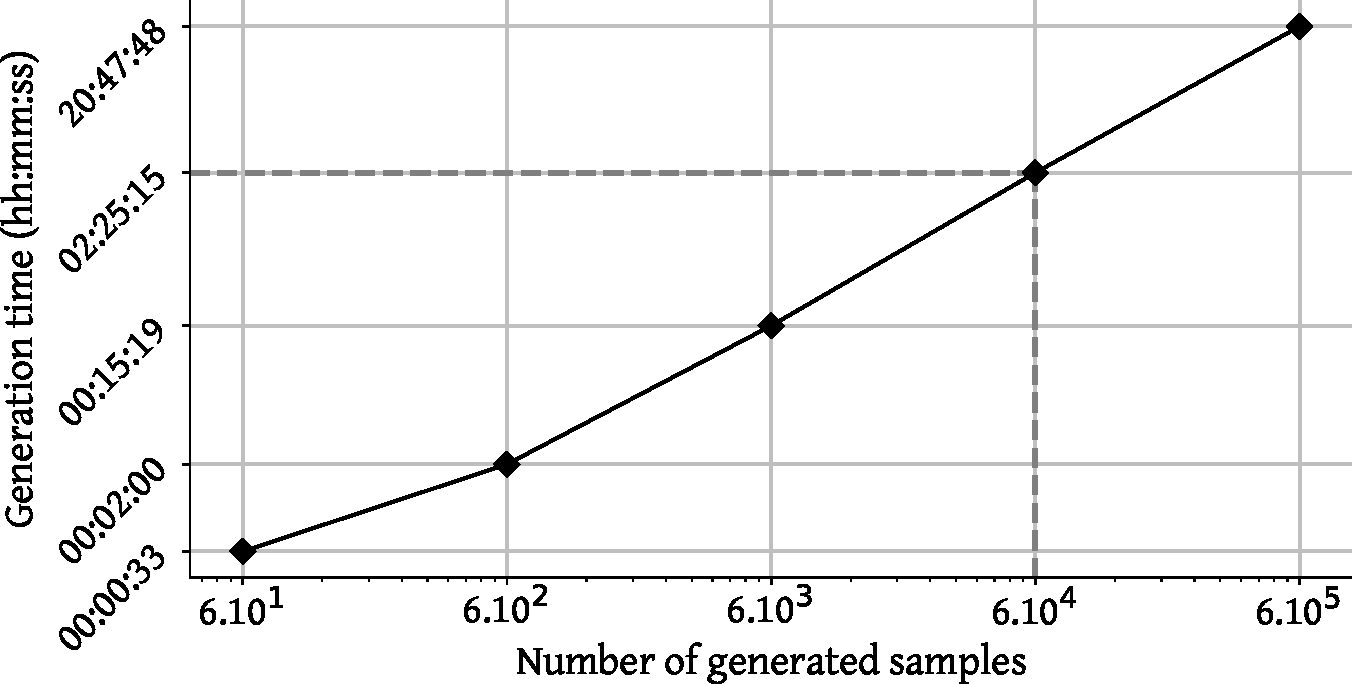
\includegraphics[width=\linewidth]{figs/topogen/generation_time.pdf}
%     \caption{Scalability of dataset generation.}
%     \label{fig:topogen-gen-time}
%   \end{subfigure}
%   \caption{\textbf{General properties of DONUT.} \textit{(a),(b)} The marginal distributions of genus and connected components are approximately uniform, ensuring balanced supervision across topological classes. \textit{(c)} The time required to generate datasets of varying sizes demonstrates that even large-scale variants remain practical.}
%   \label{fig:topogen-properties}
% \end{figure}


\subsection{Limitations and Further Improvements}

\paragraph{Topological Variety.} 
The current dataset has limited topological variety. It only encodes two characteristics: genus and number of connected components. This is mainly because all meshes are watertight and manifold. In this setting, topological invariants are trivial to deduce ($\beta_1= 2 \times \text("genus")$, $\beta_2=\beta_0$). A more challenging extension would include surfaces with boundaries, non-watertight meshes, or nested shapes. While the current generation process allows nested components in theory, no such cases are present in practice. Another direction is to incorporate families of parametric shapes with non-trivial topology, such as catenoids, helicoids, or Möbius strips.


\paragraph{Geometric Complexity.} The geometric diversity is also limited. It could be extended by adding parametric families that introduce richer geometric structures. For example, the Superformula introduced by Gielis (2003) \cite{superformula} generalizes superellipses and provides a broad range of shapes. Although we did not add such families here, since the dataset is mainly used for evaluation and no overfitting issues were observed with the current configuration, this would be valuable in other settings. In particular, if the dataset is used for pretraining, as in Point-MAE-Zero, introducing more geometric complexity would improve its utility.


